% This is file JFM2esam.tex
% first release v1.0, 20th October 1996
%       release v1.01, 29th October 1996
%       release v1.1, 25th June 1997
%       release v2.0, 27th July 2004
%       release v3.0, 16th July 2014
%   (based on JFMsampl.tex v1.3 for LaTeX2.09)
% Copyright (C) 1996, 1997, 2014 Cambridge University Press

\documentclass{jfm}
\usepackage{graphicx}
\usepackage{epstopdf, epsfig}
\usepackage{amsmath}
\usepackage{amsfonts}
\newtheorem{lemma}{Lemma}
\newtheorem{corollary}{Corollary}

% our colors
\usepackage[usenames,dvipsnames]{xcolor}
\colorlet{cesar}{red}
\colorlet{greg}{green}
\colorlet{bill}{blue}

% our packages
\usepackage{showlabels}

% hyperref
\usepackage{hyperref}
\hypersetup{
        %draft,
        breaklinks=true,
        colorlinks=true,
        linkcolor=blue,
        citecolor=Purple,
        urlcolor=Purple,
        pdfstartview={FitH},
        pdfview={FitH 0},
        pdfauthor={Cesar B. Rocha},
        pdftitle={NIWs extract energy from barotropic turbulence},
 }



%\shorttitle{ Extraction of  energy from barotropic turbulence by near-inertial waves}
\shorttitle{Near-inertial waves extract energy from barotropic turbulence}

\shortauthor{Cesar B. Rocha, Gregory L. Wagner, and William R Young}

%\title{Extraction of energy from barotropic turbulence by near-inertial waves:
%        freely-evolving flow}

\title{Near-inertial waves extract energy from barotropic turbulence:
              freely-evolving flow}
\author{Cesar B. Rocha\aff{1}
  \corresp{\email{crocha@ucsd.edu}},
  Gregory L. Wagner\aff{2}
 \and William R. Young\aff{1}}

\affiliation{\aff{1}Scripps Institution of Oceanography, University of California,
            San Diego
\aff{2}Department of Earth, Atmospheric and Planetary Sciences, Massachusetts
            Institute of Technology}

\begin{document}

\newcommand{\com}{\, ,}
\newcommand{\per}{\, .}

%% Averages
% Use \bar to over line solo symbols

\newcommand{\av}[1]{\bar{#1}}
\newcommand{\avbg}[1]{\overline{#1}}
\newcommand{\avbgg}[1]{\overline{#1}}

% A nice definition
\newcommand{\defn}{\ensuremath{\stackrel{\mathrm{def}}{=}}}

% space in equations
\newcommand{\qqand}{\qquad \text{and} \qquad}
\newcommand{\qand}{\quad \text{and} \quad}

% equations
\def\beq{\begin{equation}}
\def\eeq{\end{equation}}

\def\bea{\begin{align}}
\def\ena{\end{align}}


% calculus
\newcommand{\ord}{\mathcal{O}}
%\newcommand{\p}{\partial}
\newcommand{\ii}{{\rm i}}
\newcommand{\dd}{{\rm d}}
\newcommand{\id}{{\, \rm d}}
\newcommand{\ee}{{\rm e}}
\newcommand{\DD}{{\rm D}}
\newcommand{\wavy}{\text{wavy}}
\newcommand{\qg}{\text{qg}}
\newcommand{\dt}{\Delta t}
\newcommand{\dx}{\Delta x}
\newcommand{\be}{\beta}

\newcommand{\al}{\alpha}
\newcommand{\bx}{\boldsymbol{x}}
\newcommand{\by}{\boldsymbol{y}}
\newcommand{\bu}{\boldsymbol{u}}
\newcommand{\bv}{\boldsymbol{v}}


\newcommand{\half}{\tfrac{1}{2}}
\newcommand{\halfi}{\tfrac{\ii}{2}}
\newcommand{\quarter}{\tfrac{1}{4}}
\newcommand{\quarteri}{\tfrac{\ii}{4}}
\newcommand{\halfrho}{\tfrac{1}{2}}
\newcommand{\rz}{{}}
\newcommand{\bn}{\boldsymbol{\hat n}}
\newcommand{\br}{\boldsymbol{r}}
\newcommand{\bR}{\boldsymbol{R}}
\newcommand{\bA}{\ensuremath {\boldsymbol {A}}}
\newcommand{\bB}{\ensuremath {\boldsymbol {B}}}
\newcommand{\bU}{\ensuremath {\boldsymbol {U}}}
\newcommand{\bE}{\ensuremath {\boldsymbol {E}}}
\newcommand{\bN}{\ensuremath {\boldsymbol {\mathrm{N}}}}
\newcommand{\bJ}{\ensuremath {\boldsymbol {J}}}
\newcommand{\bXX}{\ensuremath {\boldsymbol {\mathcal{X}}}}
\newcommand{\bFF}{\ensuremath {\boldsymbol {F}}}
\newcommand{\bF}{\ensuremath {\boldsymbol {F}^{\sharp}}}
\newcommand{\bG}{\ensuremath {\boldsymbol G}}
\newcommand{\bSigma}{\ensuremath {\boldsymbol {\Sigma}}}
\newcommand{\bvarphi}{\ensuremath {\boldsymbol {\varphi}}}
\newcommand{\bxi}{\ensuremath {\boldsymbol {\xi}}}
\newcommand{\avbxi}{\overline{\ensuremath {\boldsymbol {\xi}}}}

% math cal

\newcommand{\J}{\mathcal{J}}
\newcommand{\K}{\mathcal{K}}
\newcommand{\cG}{\mathcal{G}}
\newcommand{\cF}{\mathcal{F}}
\newcommand{\cN}{\mathcal{N}}
\newcommand{\cL}{\mathcal{L}}
\newcommand{\cS}{\mathcal{S}}
\newcommand{\cE}{\mathcal{E}}


% san serif for matrices and differential operators
%\newcommand{\helmn}{\mathsf{H}_n}
\newcommand{\helmm}{\triangle_m}
\newcommand{\helmn}{\triangle_n}
\newcommand{\helms}{\triangle_s}
\newcommand{\helm}{\triangle}
\newcommand{\sA}{\mathsf{A}}
\newcommand{\sB}{\mathsf{B}}
\newcommand{\sG}{\mathsf{G}}
\newcommand{\sI}{\mathsf{I}}
%\newcommand{\sJ}{\mathsf{J}}
\newcommand{\sJ}{J}
\newcommand{\gsJ}{\breve{\mathsf{J}}}
\newcommand{\sU}{\mathsf{U}}
\newcommand{\sP}{\mathsf{P}}
\newcommand{\sQ}{\mathsf{Q}}
\newcommand{\sR}{\mathsf{R}}
\newcommand{\sL}{\mathsf{L}}
\newcommand{\Lu}{\mathsf{L}(\what{u}_k)}
\newcommand{\Nu}{\mathsf{N}(\what{u}_k)}
\renewcommand{\L}{\mathsf{L}}
\newcommand{\N}{\mathsf{N}}
\newcommand{\sH}{\mathsf{H}}
\renewcommand{\sI}{\mathsf{I}}
\renewcommand{\L}{\mathsf{L}}
\newcommand{\sM}{\mathsf{M}}
\newcommand{\sT}{\mathsf{T}}
\newcommand{\sGamma}{\mathsf{\Gamma}}
\newcommand{\sOmega}{\mathsf{\Omega}}
\newcommand{\sSigma}{\mathsf{\Omega}}
\newcommand{\sbeta}{\mathsf{\beta}}
\newcommand{\sPi}{\mathsf{\Pi}}
\newcommand{\sC}{\mathsf{C}}
\newcommand{\sQy}{\mathsf{Q}}
\renewcommand{\sb}{\mathsf{b}}

% u
\newcommand{\uhat}{\what{u}_k}

% angle brackets

\def\la{\langle}
\def\ra{\rangle}
\def\laa{\left \langle}
\def\raa{\right \rangle}


%grads and div's
%\newcommand{\bcdot}{\hspace{-0.1em} \boldsymbol{\cdot} \hspace{-0.12em}}
%\newcommand{\bnabla}{\boldsymbol{\nabla}}
\newcommand{\bnablaH}{\bnabla_{\! \mathrm{h}}}
\newcommand{\grad}{\bnabla}
\newcommand{\gradH}{\bnablaH}
\newcommand{\curl}{\bnabla \!\times\!}
\newcommand{\diver}{\bnabla \! \bcdot \! }
\newcommand{\cross}{\times}
%\newcommand{\lap}{\nabla^2}
\newcommand{\lap}{\triangle}

%varthetas and thetas
\newcommand{\vth}{\vartheta}
\newcommand{\psii}{\psi^{\mathrm{i}}}
\newcommand{\thb}{\theta^{\mathrm{-}}}
\newcommand{\vthb}{\vartheta^{\mathrm{-}}}
\newcommand{\vthbhat}{{\hat{\vartheta}}^{\mathrm{-}}}
\newcommand{\vThb}{\varTheta^{\mathrm{-}}}
\newcommand{\psib}{\psi^{\mathrm{-}}}
\newcommand{\tht}{\theta^{\mathrm{+}}}
\newcommand{\vtht}{\vartheta^{\mathrm{+}}}
\newcommand{\vththat}{{\hat{\vartheta}}^{\mathrm{+}}}
\newcommand{\vthtbhat}{{\hat{\vartheta}}^{\pm}}
\newcommand{\vTht}{\varTheta^{\mathrm{+}}}
\newcommand{\vthtb}{\vartheta^{\pm}}
\newcommand{\vThtb}{\varTheta^{\pm}}

% nondimensional numbers
\renewcommand{\Re}{\mathrm{Re}}
\newcommand{\Ro}{\mathrm{Ro}}
\newcommand{\Bu}{\mathrm{Bu}}
\newcommand{\Ri}{\mathrm{Ri}}

%psi's
%Galerking coefficient for psi:
\newcommand{\gpsi}{\breve \psi}
\newcommand{\gpsic}{{\breve \psi}^\star}
\newcommand{\gtau}{\breve \tau}
\newcommand{\gtauc}{{\breve \tau}^\star}
\newcommand{\gphi}{\breve \phi}
\newcommand{\gq}{\breve q}
\newcommand{\gU}{\breve U}
\newcommand{\gQ}{\breve Q}
\newcommand{\gsigma}{\breve \sigma}


\newcommand{\psit}{\psi^{\mathrm{+}}}
\newcommand{\psithat}{{\hat{\psi}}^{\mathrm{+}}}
\newcommand{\psibhat}{{\hat{\psi}}^{\mathrm{-}}}
\newcommand{\psitb}{\psi^{\pm}}
\newcommand{\psitbhat}{{\hat{\psi}}^\pm}
\newcommand{\St}{S^{\mathrm{+}}}
\newcommand{\Sb}{S^{\mathrm{-}}}
\newcommand{\phb}{\phi^{\mathrm{-}}}
\newcommand{\pht}{\phi^{\mathrm{+}}}
\newcommand{\tautb}{\tau^{\pm}}
\newcommand{\sigmatb}{\sigma^{\pm}}


\newcommand{\bur}{\left(\tfrac{f_0}{N}\right)^2}
\newcommand{\ibur}{\left(\tfrac{N}{f_0}\right)^2}
\newcommand{\Nm}{N_{\mathrm{mix}}}
\newcommand{\xim}{\xi_{\mathrm{mix}}}
\newcommand{\hs}{h_*}
\renewcommand{\sp}{\mathsf{p}}
\newcommand{\se}{\mathsf{e}}
\newcommand{\sptb}{\mathsf{p}^\pm}


%nmax is a problem:
%\newcommand{\nmax}{n_{\mathrm{max}}}
\newcommand{\nmax}{\mathrm{N}}
\newcommand{\mmax}{\mathrm{M}}

\newcommand{\WKB}{\mathrm{WKB}}
\newcommand{\Lam}{\Lambda}
\newcommand{\tha}{\theta}
\newcommand{\kap}{\kappa}
\newcommand{\bphi}{\boldsymbol{\phi}}
\newcommand{\third}{\tfrac{1}{3}}
\newcommand{\cs}{c^\star}
\newcommand{\dstar}{{\star\star}}
\newcommand{\nt}{n^{\mathrm{trnc}}}
\newcommand{\sDp}{\mathsf{D}^1_{\nmax}}
\newcommand{\sDpp}{\mathsf{D}^2_{\nmax}}
\newcommand{\sD}{\mathsf{D}}
\newcommand{\sDN}{\mathsf{D_\nmax}}
\newcommand{\sK}{\mathsf{K_2}}
\newcommand{\stheta}{\mathsf{\theta}}
\newcommand{\sphi}{\mathsf{\phi}}
\newcommand{\sq}{\mathsf{q}}
\newcommand{\cosech}{\text{csch}\,}
\newcommand{\sinc}{\text{sinc}\,}

%%%%%%%%% %%%%

%%%%%%%%% %%%%
\newcommand{\zt}{z^+}
\newcommand{\zb}{z^-}
\newcommand{\qA}{q^A_{\nmax}}
\newcommand{\psiB}{\psi^B_{\nmax}}
\newcommand{\phiB}{\phi^B_{\nmax}}
\newcommand{\eye}{\boldsymbol{\hat{i}}}
\newcommand{\jay}{\boldsymbol{\hat{j}}}
\newcommand{\kay}{\boldsymbol{\hat{k}}}
\newcommand{\psiG}{\psi^{\mathrm{G}}}
\newcommand{\qG}{q^{\mathrm{G}}}
\newcommand{\uG}{u^{\mathrm{G}}}
\newcommand{\UG}{U^{\mathrm{G}}}
\newcommand{\UGN}{U^{\mathrm{G}}_{\nmax}}
\newcommand{\QGN}{Q^{\mathrm{G}}_{\nmax}}
\newcommand{\sumoddn}{\sum_{n = 1, n~ \text{odd}}^{\nmax}}

% bretherton
\newcommand{\qBr}{q_{\mathrm{Br}}}
\newcommand{\psiBr}{\psi_{\mathrm{Br}}}

\newcommand{\ep}{\epsilon}
\newcommand{\vep}{\varepsilon}


%\renewcommand{\sZ}{\mathsf{Z}}
%\renewcommand{\sE}{\mathsf{E}}
\newcommand{\iBu}{\left(\tfrac{f_0}{N}\right)^2}
\newcommand{\F}{\mathcal{F}}
\newcommand{\D}{\mathcal{D}}
\newcommand{\phis}{\phi^\star}
\newcommand{\Ff}{\mathbf{F}}
\newcommand{\Sf}{\mathbf{S}}
\newcommand{\ut}{\mathbf{u}^\#}
\newcommand{\cg}{\mathbf{c}_g}
\newcommand{\Uf}{\mathbf{U}}
\renewcommand{\Im}{\mathrm{Im}}
\renewcommand{\div}{\nabla\cdot}
\renewcommand{\P}{\mathcal{P}}
\newcommand{\dU}{\delta U}
\newcommand{\W}{\mathcal{W}}
\newcommand{\cK}{\mathcal{K}}
\newcommand{\cP}{\mathcal{P}}
\renewcommand{\L}{\mathsf{L}}
\renewcommand{\N}{\mathsf{N}}
\newcommand{\psiq}{\psi^q}
\newcommand{\psiw}{\psi^w}
%\newcommand{\tfrac}{\frac}
%\newcommand{\eqref}{\ref}



\maketitle

\begin{abstract}
\end{abstract}

\begin{keywords}

\end{keywords}


\section{Introduction}

% 1) The mesoscale energy conundrum: a recalcitrant problem
The closing of the ocean's energy budget remains poorly understood, largely because
geostrophic turbulence transfers energy towards large scales.
Existing studies suggest a panoply
of ageostrophic mechanisms to account for the required forward flow of energy.
These include (but are not limited to) surface and
benthic boundary turbulence and wave generation by geostrophic eddies sloshing
over bottom topography \citep[see ][their figure 1, and references therein]{nagai_etal2015}.
But roughly half of the energy flux out of the ocean mesoscales remains unaccounted for.

% 2) Stimulated imbalance: a newish mechanism
Recent studies suggest that the interaction
of geostrophic flows with externally-forced (windy) internal waves serves
as a major sink of mesoscale energy en route to viscous dissipation
\citep{xie_vanneste2015,taylor_straub2016,wagner_young2016,barkan_etal2016}.
The emphasis on interactions of geostrophic flow with windy internal waves ---
here denoted stimulated imbalance\footnote{Following \cite{xie_vanneste2015} and
\cite{wagner_young2016} we define
\textit{stimulated imbalance} as wave-mean interactions that transfer energy from
geostrophic motions (the `mean flow') to existing internal
waves. This definition constrats with the nomenclarute recently employed by
\cite{barkan_etal2016}, who term stimulated imbalance a process by which
internal waves trigger a forward cascade from mesoscale to submesoscale (but
subinertial) flows.} ---
contrasts with energy loss via spontaneous emission --- a process by which
internal waves are emitted during geostrophic adjustment
\citep[e.g., ][]{shakespeare_hogg2017}. While spontaneous emission is localized
at sharp fronts (large Rossby number, $\Ro\gtrsim 1$) in the surface boundary
layer \citep[e.g., ][]{shakespeare_hogg2017}, stimulated imbalance operates at
the small Rossby-number ($\Ro\ll 1$), quasi-geostrophic regime, both in the upper
ocean and in the interior \citep[e.g., ][]{xie_vanneste2015}.

% 3) A minimal model of stimulated imbalance
We here study the interaction between macroturbulence and internal waves using a
simple model that contains stimulated imbalance. This minimal model is a special
family of solutions of the \cite{xie_vanneste2015} equations, which couple the
evolution of near-inertial back-rotated velocity with quasigeostrophic flow. The
focus on QG-NIW interactions is justified:  geostrophic eddies account for the
bulk of the ocean's eddy kinetic energy \cite[$90\%$,][]{ferrari_wunsch2009} and
near-inertial waves contain most of the oceanic high-frequency variability
\citep{alford_etal2016}. The minimal QG-NIW coupled model transparently reveals
the physics of stimulated imbalance associated with vertical vorticity and lateral strain.


\section{The physics of NIW energy extraction from a barotropic QG flow}

\subsection{The \cite{xie_vanneste2015} minimal QG-NIW model}

With barotropic quasigeostrophic flow, $\psi=\psi(x,y,t)$,
uniform background buoyancy frequency $N_0$, and
single-mode NIW vertical structure, $\ee^{\ii m z}$, the \cite{xie_vanneste2015}
QG-NIW coupled model (Appendix A) reduces to
\beq
\label{macroturb}
q_t + \sJ(\psi,q) = 0\com
\eeq
with the NIW-averaged quasigeostrophic potential vorticity (QGPV)
\beq
\label{qgpv}
q = \lap \psi +
                 \tfrac{1}{f_0}\Big[ \tfrac{1}{4} \lap |\phi|^2 + \tfrac{\ii}{2}
                 \sJ(\phi^\star,\phi)\Big]\com
\eeq
and the streamfunction is defined so that the geostrophic flow velocity is
$(u_e, v_e) = (-\psi_y, \psi_x)$; and
\beq
\label{waves}
\phi_t + \sJ(\psi,\phi) + \tfrac{\ii}{2}\phi\lap \psi - \tfrac{\ii}{2} f_0 \lambda^2 \lap \phi
 = 0\com
\eeq
with NIW velocity
\beq
\label{niw_velocity}
u_w+\ii v_w  =\ee^{\ii (m z - f_0 t)} \phi(x,y,t)\per
\eeq
Above,
$\phi$ is the back-rotated NIW
velocity, $\lap \defn \p_x^2 + \p_y^2$ is the horizontal laplacian,
$\sJ(f,g)=f_x g_y - f_y g_x$ is the horizontal Jacobian, and
$\lambda = \tfrac{N_0}{f_0\, m}$  is an intrinsic horizontal scale.

Similarly to the \cite{young_benjelloul1997} model, the NIW amplitude $\phi$
evolves through wave dispersion --- the last term in \eqref{waves} --- and
advection and refraction by the QG flow --- the second and third terms in
\eqref{waves}. But the wave equation \eqref{waves} is non-linear owing to the
quadratic wave terms in the \textit{inversion} relation \eqref{qgpv}. In other
words, the
\cite{young_benjelloul1997} NIW model is purely kinematic: the QG flow evolves as
if there were no waves and set an inhomonegeous medium in which NIWs propagate.
But the \cite{xie_vanneste2015} model is dynamic because both $q$ and $\phi$
determine the flow: $\psi=\psi(x,y,t; q, \phi)$. Besides advection and refraction
by the QG flow, these QG-NIW interactions imply a positive finite-amplitude
frequency shift (Appendix A).

The wave equation \eqref{waves} is similar to the reduced-gravity
Young \& Ben Jelloul model derived by  \cite{danioux_etal2015}. Without advection,
\eqref{waves} is analogous to Schrodinger's equation
\citep[e.g.,][ pg. 51]{landau_lifshitz2013}, with the vorticity playing the role
of the
potential and the dispersivity mimicking Planck's constant
\citep{danioux_etal2015}.

\subsection{Quadratic invariants and energy conversion}

From \eqref{waves}, the near-inertial kinetic energy density $\half |\phi|^2$
satisfies
\beq
\label{action_density}
\p_t \half |\phi|^2 + \sJ(\psi,\half|\phi|^2) + \diver\underbrace{\left[\tfrac{\ii}{4}
f_0\lambda^2\left(
\phi\grad\phis-\phis\grad\phi\right)\right]}_{\defn \Ff_w} = 0\per
\eeq
Locally, $\half |\phi|^2$ changes due to divergences of the geostrophic
and wave fluxes of $\half |\phi|^2$ --- the second and third terms in
\eqref{action_density}. The wave flux  $\Ff_w$ is analogous to the probability
current density of quantum mechanics (e.g., Landau \& Lifshitz, pg 57).
 Using the polar representation
$\phi = |\phi|\ee^{\ii\Theta}$ \citep[e.g., ][]{klein_etal2004}, we can compactly
express the wave flux
\beq
\label{Fw2}
\Ff_w =\tfrac{\ii}{4}f_0\lambda^2\left(\phi\grad\phis-\phis\grad\phi\right) =
f_0 \lambda^2\grad\Theta \times
\half |\phi|^2\per
\eeq
The expression on the right of \eqref{Fw2} makes it explicit that $\Ff_w$ is a
wave flux of kinetic energy density $\half|\phi|^2$, where $f_0\lambda^2\grad\Theta
= \tfrac{N^2_0}{f_0 m^2}\grad\Theta$ is the generalized group
velocity of hydrostratic NIWs, which can be quickly verified under the plane-wave
assumption $\Theta = kx + ly$.

With simple boundary conditions, e.g., periodic or no normal flux, the QG-NIW
model \eqref{macroturb}-\eqref{waves} conserves NIW kinetic energy
\beq
\label{action}
K_w \defn \half \la |\phi|^2 \ra\com
\eeq
where angle brackets, $\la \,\,\ra$, represent average over the domain of area
$\mathcal{A}$:
\beq
\label{average}
\la\, f \ra \defn \frac{1}{\mathcal{A}}\iint\limits_{\mathcal{A}} f \,\dd x \dd y\per
\eeq

Also from \eqref{waves}, we form an equation for the wave potential energy:
$\tfrac{\lambda^4}{4}\la\lap\phis\times\eqref{waves}$ + $\lap\phi\times
\eqref{waves}^\star\ra$ yields
\beq
\label{Pw}
\frac{\dd}{\dd t}\underbrace{\la\tfrac{\lambda^2}{4}|\grad \phi|^2\ra}_{P_w} =
\underbrace{\tfrac{1}{f_0}\Big\la\half\lap\psi\diver\Ff_w
\Big\ra}_{\defn\Gamma_{r}} +
\underbrace{\tfrac{\lambda^2}{2}\, \Big\la\half\left[\lap\phis\sJ(\psi,\phi)
+ \lap\phi\sJ(\psi,\phis)\right]\Big\ra}_{\defn\Gamma_a}\per
\eeq
Finally, we form an equation for the QG kinetic energy, $K_e$: $\la\psi\times
\eqref{macroturb}\ra$ in combination with \eqref{qgpv}, \eqref{action_density},
and \eqref{waves} gives
\beq
\label{Ke}
\frac{\dd}{\dd t}\underbrace{\la\half |\grad \psi|^2\ra}_{\defn K_e} =
 - (\Gamma_r + \Gamma_a) \com
\eeq
thus proving that the QG-NIW model \eqref{macroturb}-\eqref{waves} conserves
the coupled energy
\beq
\label{E}
E \defn K_e + P_w\per
\eeq
In \eqref{Ke},
$\Gamma_r + \Gamma_a$ is the energy conversion between QG kinetic energy and
wave potential energy.
The term $\Gamma_r$   stems from refraction and is easy to
interpret: the convergence, $\nabla\cdot\Ff_w < 0$, of the wave flux of NIW kinetic energy density
 into anticyclones, $\lap\psi<0$, is a source of NIW potential
energy, $P_w$.

The term $\Gamma_a$ stems from advection and is similar to the source
of variance of a trace gradient subject to lateral stirring,
\beq
c_t + \sJ(\psi,c) = 0.
\eeq
The variance production of passive scalar gradient, $\la |\grad c|^2\ra$, is
$\la\lap c \sJ(\psi,c)\ra$. Analogously,
$\Gamma_a$ is the source of NIW potential energy due to geostrophic
stirring.  After multiple
integration by parts, we rewrite this term as
\beq
\label{gradphi}
  \Gamma_a =
    \left\la
    \begin{bmatrix}
    \phi_x^\star & \phi_y^\star
    \end{bmatrix}
    \Sf
  \begin{bmatrix}
    \phi_x \\  \phi_y
    \end{bmatrix}\right\ra\com
\eeq
where $\Sf$ is the symmetric part of the geostrophic velocity gradient matrix,
\beq
\Sf \defn
\begin{bmatrix}
    -\psi_{xy} & \half(\psi_{xx} - \psi_{yy})\\
    \half(\psi_{xx}-\psi_{yy}) & \psi_{xy}
\end{bmatrix}\,\com
\eeq
whose sum of the elements squared (the Frobenius norm) is commonly defined as the
square of the QG rate of strain. Geostrophic straining enhances existing gradients
of $\phi$, thereby generating wave potential energy, $P_w$. When the QG flow has
a lateral scale much larger than
the NIW field, this distortion of $\phi$ is akin to the wave-capture
mechanism of \cite{buhler_mcintyre2005}.

%An important caveat to this analogy is that the NIW amplitude $\phi$ is dynamically active.
%The explicit expression for the conversion
%$\Gamma$ nicely shows that non-trivial barotropic QG-NIW interaction requires
%geostrophic vorticity or strain (or both).

\subsection{Averaged equations and loss of coherence}
The domain-averaged potential vorticity $\la q \ra$ is invariant as a consequence of
the material invariance of $q$ --- or the invariance of the average of each
individual term in \eqref{qgpv}. The spatially-averaged (coherent) NIW amplitude
satisfies
\beq
\label{phi_ave}
\frac{\dd}{\dd t}\la \phi \ra + \ii \left\la\half\phi\lap\psi \right\ra = 0\per
\eeq
Introducing the decomposition $\phi = \la\phi\ra+\phi'$, we have
\beq
\half\la|\phi|^2\ra
= \underbrace{\half|\la\phi\ra|^2}_{\defn K^c_w} +
\underbrace{\half\la|\phi'|^2\ra}_{\defn K^i_w}\com
\eeq
Thus, the kinetic energy of horizontally incoherent ($\phi'$) and coherent
($\la\phi\ra$) NIW amplitude satisfy
\beq
\label{Kiw}
\dot{K}_w^i = \Pi\com
\eeq
and
\beq
\label{Kcw}
\dot{K}_w^c = -\Pi\com
\eeq
with the kinetic energy transfer
\beq
\label{Pi}
\Pi = \tfrac{\ii}{2}\left[\la\half\phi\lap\psi\ra\la\phis\ra -
\la\half\phis\lap\psi\ra\la\phi\ra\right]\per
\eeq
The decay of a laterally coherent near-inertial oscillation due to refraction by
geostrophic flow is relevant for mixed-layer slab models used to estimate the work
imparted by wind into the NIW field \citep[e.g., ][]{alford2001}. Without further
assumptions, it is unclear if the effect of refraction is sign definite. If the
NIWs have initial larger scales than the geostrophic field, then refraction
generates eddy-scale perturbations, implying a reduction of lateral coherence
($\Pi > 0$). But it remains unclear if this transfer can be parameterized as a linear
damping.

\subsection{Relevant parameters}
Using the scaling
\beq
\psi \sim U_e k_e^{-1} \com\qquad \text{and} \qquad \phi \sim U_w\com
\eeq
with characteristic QG and NIW velocity scales $U_e$ and $U_w$, and the
characteristic horizontal length scale $k_e^{-1}$ and time scale $(U_e k_e)^{-1}$,
reveals that there are two dynamically relevant parameters of the QG-NIW problem
described by \eqref{macroturb}-\eqref{waves}. First, the `wave amplitude'
\beq
\label{alpha}
\alpha \defn \underbrace{\frac{U_e k_e}{f_0}}_{\defn Ro} \times
\underbrace{\left(\frac{U_w}{U_e}\right)^2}_{\defn \ep^2}\com
\eeq
measures the strenght of the waves compared to the geostrophic flow and scales
the contribution of the NIW terms to the QGPV.
Second, the `wave dispersivity,'
\beq
\label{hslash}
\hslash \defn f_0 \lambda^2 \times \frac{k_e}{U_e}\com
\eeq
scales the importance of linear dispersion, which counteracts the unsmoothing
effects of advection and refraction.

Also, the two conversion terms, $\Gamma_r$ and $\Gamma_a$,
scale with the same non-dimensional parameter $\alpha\times \hslash$. But this
does not imply that the energy conversion scales linearly with both wave amplitude
and dispersivity: the scales deloveped by the NIW amplitude field $\phi$ and the
 correlations in $\Gamma$ depend on $\alpha$ and $\hslash$


\subsection{Summary}
We can summarize the physics of stimulated imbalance considering an initial value
problem that idealizes the oceanographic `post-storm' context: stormy winds impart momentum
into the ocean, thereby generating near-inertial oscillations with a lateral
decorrelation scale larger than the mesoscale eddies. The after-storm evolution
of an initially large-scale coherent inertial oscillation is described by
\eqref{macroturb}--\eqref{waves} \citep{xie_vanneste2015}. Geostrophic refraction
focus NIWs in anticyclones. The eddy-scale gradients of $\phi$ then support
geostrophic advection. Advection and refraction reduce the lateral coherence
of NIWs --- and wave dispersion counteracts this unsmoothing effect.

The explicit expression for energy
conversion on the right of \eqref{Pw} enlightens the physics of  the problem.
Refraction causes a convergence of NIW kinetic energy density in anticyclones.
And advection strains the NIW field, enhancing the gradients of $\phi$. Both
processes generate NIW potential energy at the expenses of geostrophic kinetic
energy, thus motivating the nomenclature `refraction sink' ($-\Gamma_r$) and
`advection sink' ($-\Gamma_a$)  of QG kinetic energy.

The remaining of this paper verifies this thought experiment by solving
numerically two problems in which an initially perfectly coherent near-inertial
oscillation interacts with the Lamb dipole (Section 3) and with a turbulent
field emergent from random initial conditions (Section 4).

\section{The Lamb-Chaplygin dipole}
The Lamb-Chaplygin dipole is an exact solution of the Euler
equations on an infinite two-dimensional plane where the vorticity is confined
to a circle of radius $R$ \cite[][]{meleshko_vanheijst1994}. The solution, steady on a frame moving at uniform zonal
velocity $U$, is
\beq
\label{lambd_q}
  \lap\psi =
     \frac{2 U \kappa}{J_0(\kappa R)} \begin{cases}
      J_1(\kappa r)\sin\theta\com & \text{if}
      \qquad r\le R\com\\
      0\com &\text{if} \qquad r\ge R\com
  \end{cases}
\eeq
where $r^2 = (x-x_c)^2+(y-y_c)^2$ is the radial distance about the dipole's center
$(x_c,y_c)$, $\tan \theta = (y-y_c)/(x-x_c)$, and $J_n$ is the n'th order Bessel
function of first kind. The matching condition at $r=R$, $J_1(\kappa R)=0$, determines
$\kappa$. The dipole is the first eigensolution, with eigenvalue $\kappa R \approx
3.8287$.  If the wave QGPV is zero, then the dipole \eqref{lambd_q} is a
solution of \eqref{macroturb}. This is the case when a uniform $\phi$ is used as
initial condition (Sections 3 and 4). Dipole images, an artefact of periodization,
cause a small zonal drift of the dipole. This effect is negligible in our
examples below because the dipole is confined to a region much smaller than the
domain size $L$: $R/L = 0.1$.

While we perform the calculations with dimensional variables, we non-dimensionalize
the results for clarity. For the dipole \eqref{lambd_q}, we use  $U_e = U$ and
$k_e = 2\pi/R$. As for the initial NIW amplitude, we consider a uniform (i.e.,
perfectly  coherent) near-inertial oscillation with speed $U_w$:
\beq
\label{NIO}
\phi(x,y,t=0) = \tfrac{1 + \ii}{\sqrt{2}}\, U_w\per
\eeq

\subsection{Solution for $\hslash \approx 1$ and $\alpha \approx 3.75$}

The wave concentration in anticylones is quantified by the correlation coefficient
\citep[e.g., ][]{danioux_etal2015}
\beq
\label{corr_r}
r \defn \frac{\left\la |\phi'|^2\,\lap\psi\right\ra}{
\left\la |\phi'|^4\right\ra^{1/2} \left\la (\lap \psi)^2\right\ra^{1/2}}\per
\eeq

\begin{figure}
\centering
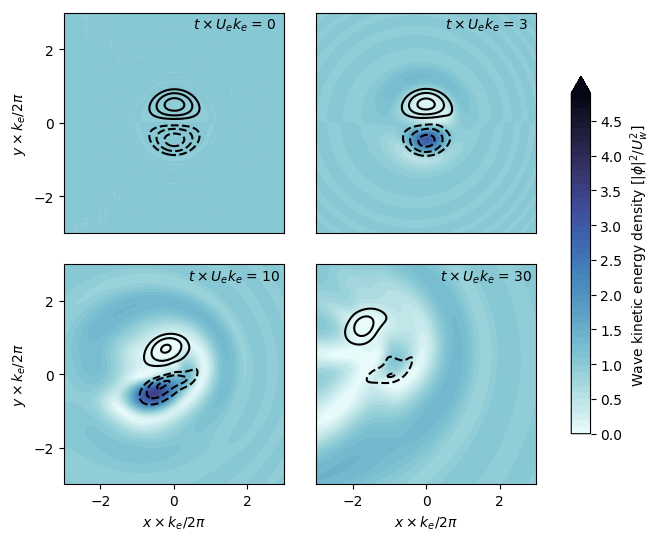
\includegraphics[width=.925\textwidth]{figs/fig1.png}
\caption{Snapshots of the Lamb-Chaplygin dipole solution with $\hslash \approx 1$
        and $\alpha \approx 3.75$. Colors represent wave kinetic energy density,
         $|\phi'|^2/U_w^2$.
        Contours represent potential vorticity, $q\times U_e k_e = [
        -1.5,-0.5,1.5,0.5]$, with dashed lines showing negative values.
        These plots only show the central $\tfrac{1}{5}\times\tfrac{1}{5}$
        subdomain.}
\end{figure}

\begin{figure}
\centering
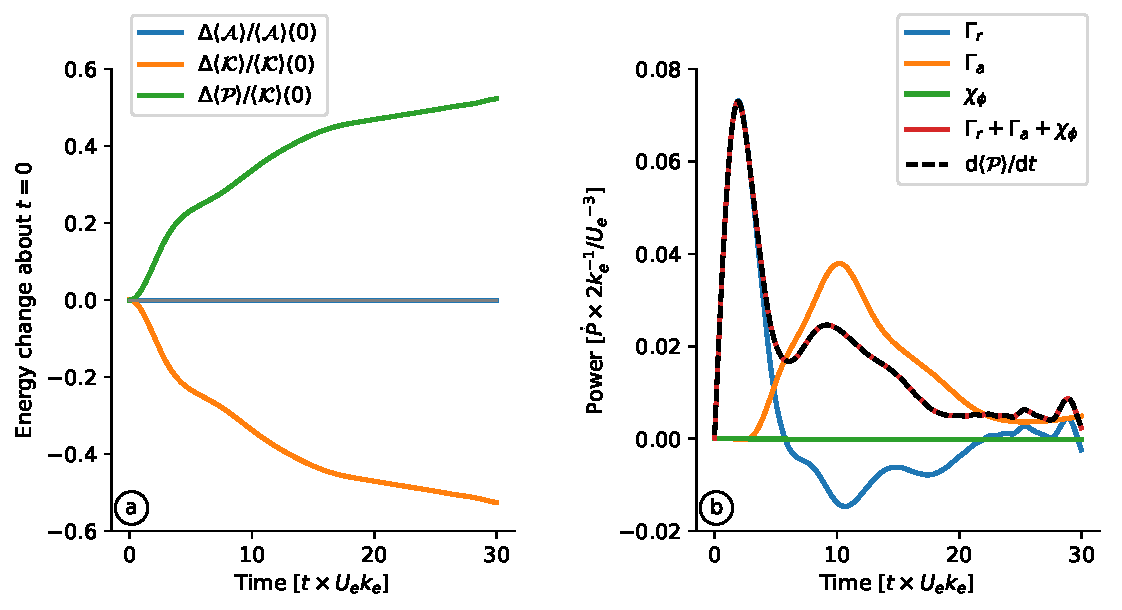
\includegraphics[width=1.\textwidth]{figs/fig2.pdf}
\caption{Statistics of the Lamb-Chaplygin dipole solution with $\hslash \approx 1$
        and $\alpha \approx 3.75$. (a) Energy change about initial condition.
        (b) Wave potential energy budget \eqref{Pw}. (c) Incoherent wave kinetic
        energy budget \eqref{Kiw}. (d) Coeficient of correlation between
        incoherent wave
        kinetic energy and relative vorticity \eqref{corr_r}.
        }
\end{figure}

\section{Decaying Macroturbulence}

To study the QG-NIW interaction and energy exchange in a turbulent regime relevant
to the ocean, we consider a barotropic turbulence flow that emerges from
random initial conditions integrated for 20 eddy turnover time units.
In other words, we first integrate the initial condition
\beq
\label{psi_init}
\psi \big(x,y, t \times U_e k_e = -20\big) = \sum_{k,l} |\hat{\psi}|\cos\left(k x + l y +
\chi_{k,l}\right)
\eeq
with waveless QG dynamics before introducing waves at $t\times U_e k_e = 0$.
In \ref{psi_init}, $\chi_{k,l}$ is a random phase uniformly distributed on $[0, 2\pi)$,
 and $|\hat\psi|$ is the isotropic spectrum
\beq
\label{psih_mag}
|\hat{\psi}| = C \times \big\{|k|\,[1 + (|k|/k_e)^4]\big\}^{-1/2}\com
\eeq
with the wavenumber magnitude $|k|^2 = k^2 + l^2$. The prescribed initial energy
$U_e^2/2$ determines the constant C:
\beq
\label{ke_init}
\sum_{k,l} \underbrace{|k|^2 |\hat{\psi}|^2}_{\defn \cK_e} = \tfrac{1}{2}U_e^2\per
\eeq
The kinetic energy spectrum $\cK_e$ peaks at the energy-containing scale $k_e^{-1}$.
At scales smaller than $k_e^{-1}$, $\cK_e$ has a linear dependence in $|k|$,
whereas it decays as $|k|^{-3}$ at scales larger than $k_e^{-1}$. This red spectrum
ensures insignificant energy dissipation by the biharmonic viscosity added to
 \eqref{macroturb} to absorb the forward cascade of enstrophy (Appendix B).

 The evolution of a random initial condition constrained by the inviscid
 dynamics \eqref{macroturb} has been well studied, beginning with \cite{fornberg1977}.
 Stirring of vorticity $\lap \psi$ by the flow $\psi$ transfers enstrophy towards
 small scales; energy flows to large
 scales. Most of enstrophy dissipated within few eddy turnover time units, whereas
 kinetic energy is nearly conserved. Vorticity concentrates into localized
 structures: after 20 eddy turnover time units, the vorticity is well-organized
 into a sea of coherent vortices that form via like-sign vortex merging
 \citep[e.g., ][]{mcwilliams1984}.

 We add a perfectly coherent near-inertial oscillation \eqref{NIO} to the mature
 barotropic turbulence at $t \times U_e k_e = 0$. For all parameters considered
 in the remaing of this paper, there are no qualitative long-term differences
 between the solutions described below and results from introducing the waves
 at $t\times U_e k_e = -20$.



\subsection{Parameters for strong mid-latitude macroturbulence}

Consider strong mid-latitude macroturbulence, such as the Gulf Stream or Kuroshio
Extension. The choice of parameters, $U_e = 0.1$ m s$^{-1}$,
$f_0 = 1 \times 10^{-4}$ s$^{-1}$, $2\pi k_e^{-1} = 125$ km
gives a Rossby number $Ro \approx  0.05$. For reference, the eddy-turnover scale
is $(U_e k_e)^{-1}\approx 5.8\,\,\text{days}$. Strong NIW velocity imparted by
atmospheric storms, $U_w \sim \sqrt{2} U_e$, implies a wave amplitude
\beq
  \alpha \approx 0.1\per
\eeq
A NIW vertical wavelength of $\lambda_z = 2\pi/m = 300$ m \citep[e.g., ][]{alford_etal2016}
on a strongly stratified upper-ocean $N_0/f_0 = 100$ yields a dispersivity
\beq
  \hslash \approx 1.0 \per
\eeq

\subsection{Solutions for $\hslash = 1$ and $\alpha = 0.1$}

\subsection{Parameter exploration}

\section{Final Remarks}

\appendix

\section{Details of the QG-NIW model}

\subsection{The \cite{xie_vanneste2015} model}
\cite{xie_vanneste2015} derive the QG-NIW model using a variational formulation
of the generalized Lagrangian mean (GLM) framework with Whitham averaging.
Following \cite{young_benjelloul1997}, Xie \& Vanneste write the
NIW velocity in complex form
\beq
u_w + \ii v_w = M_z \ee^{-\ii f_0 t}\per
\eeq
Their derivation recovers the wave equation that governs the
evolution of the NIW complex amplitude $M_z$
\beq
M_{zzt} + \p_z \sJ(\psi,M_{z}) + \tfrac{\ii}{2}\left[\left(\frac{N^2}{f_0}+\psi_{zz}
\right)\lap M - 2 \nabla\psi_z\cdot\nabla M_z + M_{zz}(\lap\psi + 2 \beta y) \right] = 0 \com
\eeq
with the QG streamfunction $\psi(x,y,z,t)$. The QG flow evolves through stirring of QGPV
\beq
q_t + \sJ(\psi,q) = 0\per
\eeq
A fundamental difference is that the QGPV in the \cite{xie_vanneste2015}
model contains quadratic wave terms
\beq
q = \nabla \psi + \left(\tfrac{f_0^2}{N^2}\psi_z\right)_z + \beta y +
    \tfrac{\ii}{2 f_0}\sJ(M_z^\star,M_z) + \tfrac{1}{4f_0}\left(
    2 |\nabla M_z|^2 - M_{zz}^\star\nabla M - M_{zz}\nabla M^\star\right)\per
\eeq
Thus the NIWs actively evolve, feedbacking onto the QG flow.
The model of \cite{xie_vanneste2015}, with the potential vorticity that includes
wave terms, generalizes early ideas introduced by
 \cite{buhler_mcintyre1998}  to a setup that avoids spatial scale separation between
 geostrophic flow and waves, but restricts attention to near-inertial frequencies.
Using standard perturbation theory, \cite{wagner_young2016} contemporarily
recovered and extended this coupled QG-NIW system.

The special family of solutions with barotropic, f-plane QG flow, uniform background
stratification, and single vertical mode NIW, $M_z = \ee^{\ii m z}\phi(x,y)$,
yields the reduced set of equations \eqref{macroturb}-\eqref{waves} used
in this paper.


% \subsection{Energy conservation}
% We obtain the energy conservation for the minimal QG-NIW model by inserting
% the barotropic flow $\psi$, uniform stratification, and single-vertical mode
% solution into the conservation laws derived by \cite{xie_vanneste2015} and
% \cite{wagner_young2016}. Alternatively, we can deduce these conservation alaws
% from the model equations \eqref{macroturb}-\eqref{waves}. Throughout we
% use --- sometimes relentlessly --- integration by parts and
% assume no normal flux or periodic boundary conditions.

% First, we form an equation for the NIW kinetic energy density: $\phis\times
% \eqref{waves} + \phi\times\eqref{waves}^\star$ yields \eqref{action_density}.
% Averaging this density equation gives the conservation of NIW kinetic energy
% $K_w = \half \la|\phi|^2\ra$, with the horizontal average of the domain of area
% $\mathcal{A}$:
% \beq
% \label{average}
% \la\, f \ra \defn \frac{1}{\mathcal{A}}\iint\limits_{\mathcal{A}} f \,\dd x \dd y\per
% \eeq
% More generally, NIW action is conserved in the QG-NIW model
% \citep[e.g., ][]{wagner_young2016}, but in the $f-$plane reduced set
% \eqref{macroturb}-\eqref{waves}, the difference between $K_w$ and NIW action is
% a mere constant $f_0$. We can re-write the expression for the wave flux of kinetic
% energy density using the polar representation $\phi = |\phi|\ee^{\ii\Theta}$
% \citep[e.g., ][]{klein_etal2004}:
% \beq
% \label{Fw2}
% \Ff_w =\tfrac{\ii}{4}f_0\lambda^2\left(\phi\grad\phis-\phis\grad\phi\right) =
% f_0 \lambda^2\grad\Theta \times
% \half |\phi|^2\per
% \eeq
% The expression on the right of \eqref{Fw2} makes it explicit that $\Ff_w$ is a
% wave flux of kinetic energy density $\half|\phi|^2$, where $f_0\lambda^2\grad\Theta
% = \tfrac{N^2_0}{f_0 m^2}\grad\Theta$ is the generalized group
% velocity of hydrostratic NIWs, which can be quickly verified under the plane-wave
% assumption $\Theta = kx + ly$.
%
% Next, we form an equation for the NIW potential energy $P_w$:
% $\tfrac{\lambda^4}{4}\la\lap\phis\times\eqref{waves}$ + $\lap\phi\times
% \eqref{waves}^\star\ra$ yields
% \beq
% \label{Pw}
% \dot{P}_w = \underbrace{\tfrac{1}{f_0}\Big\la\half\lap\psi\diver\Ff_w
% \Big\ra}_{\Gamma_{r}} +
% \underbrace{\tfrac{\lambda^2}{2}\, \Big\la\half\left[\lap\phis\sJ(\psi,\phi)
% + \lap\phi\sJ(\psi,\phis)\right]\Big\ra}_{\Gamma_a}\per
% \eeq
% Finally, we form an equation for the QG kinetic energy $K_e$: $\la\psi\times
% \eqref{macroturb}\ra$ in combination with \eqref{qgpv}, \eqref{action_density},
% and \eqref{waves} yields $\dot{K}_e = - (\Gamma_r + \Gamma_a)$, thus proving the
% conservation of energy $E = K_e + P_w $.
%
% \subsection{Energy conversion}
% Neither term of the energy conversion $\Gamma = \Gamma_r + \Gamma_a$ is sign
% definite. However, the bulk of the conversion is positive ($K_e \to P_w$) in all
% numerical simulations. The first term is the easiest to interpret:
% refraction of NIWs by the QG vorticity causes a convergence of NIW kinetic energy
% density ($\diver\Ff_w<0$) in regions of negative vorticity ($\lap\psi<0$), thus
% $\Gamma_r > 0$. To interpret the second term $\Gamma_a$, we consider the equation
% of a passive scalar c:
% \beq
% \label{passive}
% c_t + \sJ(\psi,c) = 0\per
% \eeq
% To form an equation for the variance of the passive scalar gradient, we perform
% an operation analogous to that used in deriving the equation for $P_w$: $ \la\lap
% c \times \eqref{passive}\ra$ yields
% \begin{align}
% \label{gradc}
%     \p_t\la|\grad c|^2\ra &= \la\lap c \sJ(\psi, c)\ra\nonumber\\
%                                   & =
%     \left\la
%     \begin{bmatrix}
%     c_x & c_y
%     \end{bmatrix}
%     \Sf
%   \begin{bmatrix}
%     c_x \\  c_y
%     \end{bmatrix}\right\ra\com
% \end{align}
% where $\Sf$ is the symmetric part of the geostrophic velocity gradient matrix,
% \beq
% \Sf \defn
% \begin{bmatrix}
%     -\psi_{xy} & \half(\psi_{xx} - \psi_{yy})\\
%     \half(\psi_{xx}-\psi_{yy}) & \psi_{xy}
% \end{bmatrix}\,\com
% \eeq
% whose sum of the elements squared (the Frobenius norm) is commonly defined as the
% square of the QG rate of strain. In general, given an initial gradient $\grad c$,
% QG straining enhances $|\grad c|$: $\la \lap c \sJ(\psi,c) \ra$ represents the
% variance production of passive scalar gradient $\la |\grad c|^2\ra$. Analogously,
% $\Gamma_a$ is the source of NIW potential energy $P_w$ due to geostrophic
% straining. An important caveat to this analogy is that the NIW amplitude $\phi$
% is dynamically active.


\subsection{Wave self-interaction and frequency shift}
To gain further insight into the dynamics, we decompose the balanced flow
into `vorticity-induced' and `wave-induced' fields, $\psi = \psiq + \psiw$, where
\beq
\label{q_qw}
    \lap\psiq = q\com\qquad\text{and}\qquad \lap\psiw =-\frac{1}{4f_0}\lap|\phi|^2
     - \tfrac{\ii}{2f_0}\sJ(\phis,\phi)\per
\eeq
With the \eqref{q_qw} decomposition, the QGPV equation \eqref{macroturb} becomes
\beq
\label{lpsiq_t}
\lap\psiq_t + \sJ(\psiq+\psiw,\lap\psiq) = 0\per
\eeq
In other words, the relative vorticity of the `vorticity-induced' flow changes
due to advection by the total flow $\psiq+\psiw$. The wave equation satisfies
\beq
\label{waves2}
\underbrace{\left(\p_t - \tfrac{\ii}{2} f_0\lambda^2\lap\right)\phi}_{\text{Lin.
wave dynamics}} + \underbrace{\sJ(\psiw,\phi) +\tfrac{\ii}{2}\phi\lap\psiw}_{
\text{Non-lin. wave dynamics}} +\,\, \underbrace{\sJ(\psiq,\phi)+\tfrac{\ii}{2}
\phi\lap\psiq}_{\text{Adv./refrac. by } \psiq}  = 0\per
\eeq
From \eqref{q_qw}, the `wave-induced' streamfunction $\psiw$ is quadratic in $\phi$:
\beq
\label{psiw}
\psiw = \tfrac{1}{4f_0}|\phi|^2 + \tfrac{\ii}{2f_0}\lap^{-1}\sJ(\phis,\phi)\com
\eeq
where $\lap^{-1}$ is the inverse of the Laplacian: $\lap^{-1}\lap f = f $.

Together, equations \eqref{waves2}-\eqref{psiw} show the non-linear
nature of the wave equation in this coupled QG-NIW model. In particular, the
non-linear wave dynamics is cubic in wave amplitude.  Dropping these cubic
wave terms yields a quasi-linear (QL) QG-NIW system. This
QL system conserves the energy
\beq
E_{ql} \defn \la\half|\grad\psi^q|^2\ra + \la\grad\psi^q\cdot\grad\psi^w\ra +
          \la\tfrac{\lambda^2}{4}|\grad\phi|^2\ra\per
\eeq
Note that   E = $E_{ql} + \la\half|\grad\psi^w|^2\ra$. Thus, the QL approximation
is an intermediate model between the uncoupled QG-YBJ model ($\psi^w=0$)
and the non-linear coupled QG-NIW model.

To  study the non-linear wave effects, we linearize the QG-NIW equations  about
 the exact solution
$\phi = \Phi = \text{constant}$ and $\psi = 0$, so that $q=0$. The QGPV
equation \eqref{macroturb} linearized about this state is trivial: $q_t =
\lap\psiq_t = 0$, thus $\lap\psiq$ remains zero. Also,
\beq
\label{lin_q}
\lap\psiw = -\tfrac{\Phi}{2f_0}\lap\half(\phi + \phis)\com
\eeq
where $\phi$ represents the small departure about the constant $\Phi$, so that
the linearized wave equation becomes
\beq
\phi_t = \tfrac{\ii}{2}\left[\tfrac{\Phi^2}{2f_0}\lap\half(\phi+\phis) +
f_0\lambda^2\lap\phi\right] \per
\eeq
Recalling that $u_w + \ii v_w = \phi \ee^{\ii (mz -f_0 t)}$, we recast the wave
equation:
\beq
\left[\p_t^2 - \tfrac{1}{4}f_0\lambda^2\left(f_0\lambda^2+
\frac{\Phi^2}{2f_0}\right)\lap^2\right] v_w = 0\com
\eeq
where $\lap^2 = (\p_x^2 + \p_y^2)^2$. Hence, plane-wave solutions yield the
dispersion relation
\beq
\omega = \half f_0\lambda^2(k^2+l^2)\left[1+\half\tfrac{\Phi^2}{f_0^2\lambda^2}
\right]^{1/2}\com
\eeq
and we conclude that the wave self-interaction shifts the frequency by
\beq
\left[1+\half\tfrac{\Phi^2}{f_0^2\lambda^2}\right]^{1/2}-1\per
\eeq


\section{Details of the initial value problems}

\subsection{Numerical methods}
We solve the QG-NIW system \eqref{macroturb}-\eqref{waves} using a standard
collocation Fourier spectral method.
In the pseudo-spectral spirit, we evaluate  the quadratic non-linearities in
physical space, and transform the product into Fourier space. For small-scale
dissipation, we use biharmonic viscosity. We find that this choice, originally
used in \cite{mcwilliams1984}, is sufficient
to extend the spectral resolution compared to Laplacian viscosity.
We make sure the 35$\%$ highest modes fall in the dissipation range, so that alised
wavenumbers are strongly damped. We time march the spectral equations
using an exponential time differencing method with a fourth order Runge-Kutta scheme
\citep[details in][]{kassam_trefethen2005}.

\subsection{Parameters}

\begin{table}
 \begin{center}
   \caption{Description of parameters of Lamb-Chaplygin simulation.}
   \label{parameters_lamb}
   \begin{tabular}{ c | c | c }
     \hline
      Parameter & Description & Value\\
      \hline
      $\mathsf{N}$   & Number of modes &  512 \\
      $L_d$ & Domain size & $2\pi\times 200$ km \\
      $2\pi k_e^{-1}$ & Dipole radius & $L/15 \approx 84$ km \\
      $U_e$ & Dipole strength & $5\times 10^{-2}$ m s$^{-1}$ \\
      $U_w$ & NIW speed & $5\times 10^{-1}$ m s$^{-1}$ \\
      $N_0$ & Buoyancy frequency & $5 \times 10^{-3}$ s$^{-1}$\\
      $f_0$ & Colioris frequency & 10$^{-4}$ s$^{-1}$\\
      $2\pi$m$^{-1}$ & NIW vertical wavelength & $325$ m \\
      $\nu_e$ & QGPV biharmonic viscosity & $5\times 10^{7}$ m$^4$ s$^{-1}$\\
      $\nu_w$ & NIW biharmonic viscosity & $ 5 \times 10^{7}$ m$^4$ s$^{-1}$\\
   \end{tabular}
 \end{center}
\end{table}


%\begin{table}
%  \begin{center}
%    \label{parameters_description}
%    \caption{Description of parameters of numerical simulations.}
%    \begin{tabular}{ c | c | c }
%       Parameter & Description & Value \\ \hline
%       $\mathsf{N}$   & Number of modes &  512 \\
%       $L_d$ & Domain size & $2\pi\times 200$ km \\
%       $2\pi k_e^{-1}$ & Centroid wavelength & $2\pi\times 50$ km \\
%       $U_e$ & RMS velocity & $0.1$ m s$^{-1}$ \\
%       $U_w$ & NIW speed & $0.07 - 0.32$ m s$^{-1}$ \\
%       $N_0$ & Buoyancy frequency & 10$^{-2}$ s$^{-1}$\\
%       $f_0$ & Colioris frequency & 10$^{-4}$ s$^{-1}$\\
%       $2\pi$m$^{-1}$ & NIW vertical wavelength & $222 - 888$ m \\
%       $\nu_e$ & QGPV biharmonic viscosity & $5\times 10^{7}$ m$^4$ s$^{-1}$\\
%       $\nu_w$ & NIW biharmonic viscosity & $ 1 \times 10^{6}$ m$^4$ s$^{-1}$\\
%    \end{tabular}
%  \end{center}
%\end{table}



\bibliographystyle{jfm}
% Note the spaces between the initials
\bibliography{RochaWagnerYoung}

\end{document}
